\chapter{การควบคุมศัตรูพืชทางชีวภาพ (Biocontrol) และกลไกปฏิปักษ์}
\label{ch:biocontrol}

\begin{keyconcept}[แนวคิดสำคัญของบทที่ 5]
การควบคุมศัตรูพืชและโรคพืชโดยชีววิธี (Biological Control: Biocontrol)\index{การควบคุมทางชีววิธี (Biocontrol)} เป็นรากฐานสำคัญของระบบเกษตรนิเวศและความมั่นคงทางอาหารยุคใหม่ เป็นการใช้สิ่งมีชีวิตที่เป็นประโยชน์หรือสารสกัดชีวภาพจากจุลินทรีย์ปฏิปักษ์ เพื่อควบคุมประชากรแมลงศัตรูพืชและเชื้อก่อโรคให้อยู่ต่ำกว่าระดับที่ก่อความเสียหายทางเศรษฐกิจ (Economic Injury Level: EIL) กลไกของจุลินทรีย์ควบคุมโรคและแมลงมีความจำเพาะเจาะจงระดับโมเลกุลสูงมาก ตั้งแต่โครงสร้างผลึกโปรตีน Cry และ Cyt ของ \organism{Bacillus thuringiensis}\index{Bacillus thuringiensis@\textit{Bacillus thuringiensis} (Bt)} ที่เจาะรูสลายเซลล์เยื่อบุทางเดินอาหารแมลง เอนไซม์ย่อยผนังเซลล์รา (CWDEs) และสารเปปไทด์ต้านเชื้อราของ \organism{Trichoderma}\index{Trichoderma@\textit{Trichoderma}} ตลอดจนสารไลโปเปปไทด์วงแหวน (Surfactin, Iturin, Fengycin)\index{สารประกอบไลโปเปปไทด์ (Lipopeptides)} ของ \organism{Bacillus subtilis} และการเจาะเกราะไคตินของเชื้อรากำจัดแมลง \organism{Beauveria bassiana}\index{Beauveria bassiana@\textit{Beauveria bassiana}} และ \organism{Metarhizium anisopliae}\index{Metarhizium anisopliae@\textit{Metarhizium anisopliae}}
\end{keyconcept}

\begin{figure}[ht]
    \centering
    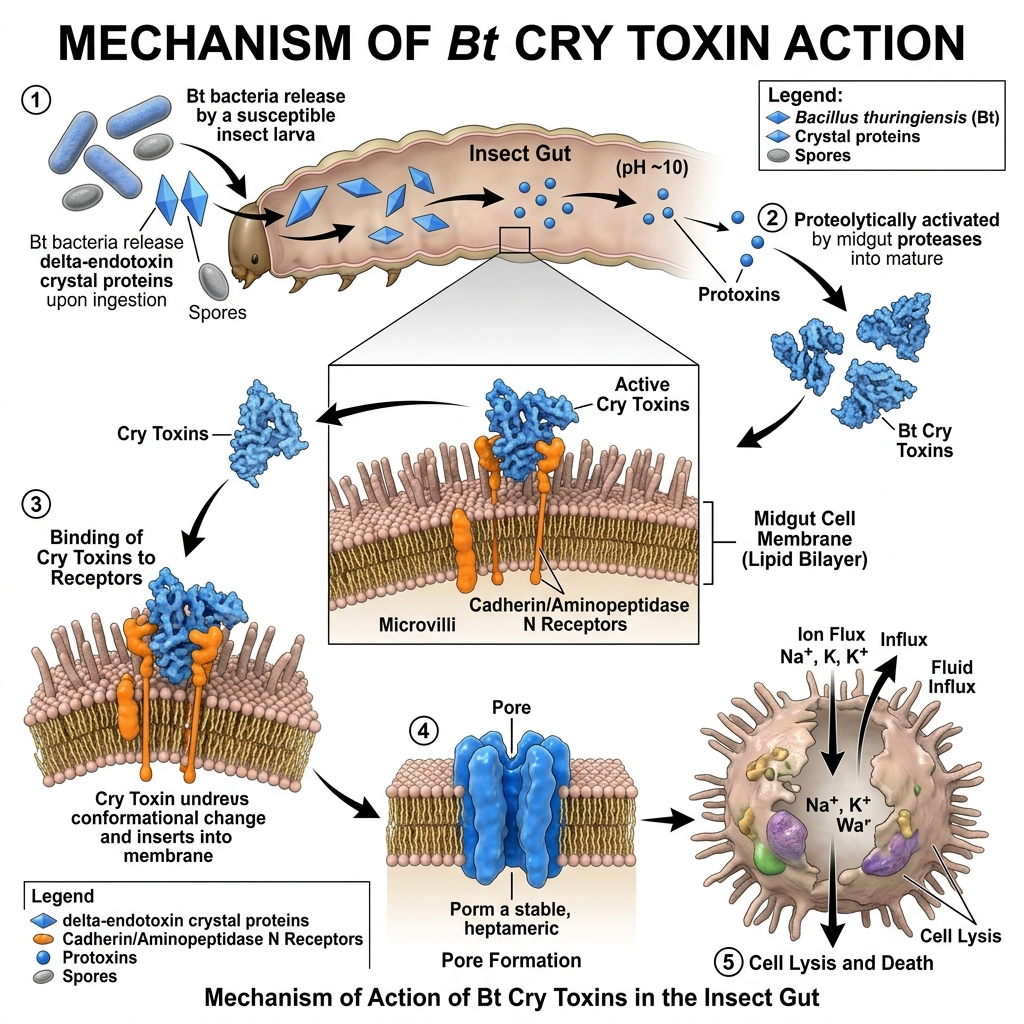
\includegraphics[width=0.85\textwidth]{assets/ch05_bt_mechanism.png}
    \caption{การจำลองภาพ 3D ขยายแสดงกลไกการทำลายของผลึกสารพิษเดลตา-เอนโดท็อกซิน (Delta-endotoxin: Cry toxin) ของแบคทีเรีย Bt ในลำไส้ส่วนกลางของหนอนแมลงศัตรูพืช แสดงขั้นตอนการหลอมละลายผลึกในสภาวะด่างจัด การตัดแต่งโมเลกุลด้วยเอนไซม์โปรติเอส การเข้าจับกับตัวรับ Cadherin และการรวมกลุ่มแทรกตัวสร้างรูรั่วทะลวงเยื่อหุ้มเซลล์ (Pore Formation) จนเซลล์แตกสลาย}
    \label{fig:ch05_bt_mechanism}
\end{figure}

\section*{วัตถุประสงค์การเรียนรู้ประจำบท}
เมื่อศึกษาบทเรียนนี้จบแล้ว นักศึกษาสามารถ:
\begin{enumerate}
    \item อธิบายโครงสร้างระดับ 3 มิติ และลำดับการออกฤทธิ์ทางชีวเคมีของโปรตีนสารพิษ Cry และ Cyt จาก \organism{Bacillus thuringiensis}
    \item วิเคราะห์กลไกปฏิปักษ์ 4 ด้านของเชื้อรา \organism{Trichoderma} spp. (Mycoparasitism, Antibiosis, Competition, Induced Resistance)
    \item อธิบายโครงสร้างและบทบาทของสารไลโปเปปไทด์วงแหวน (Surfactin, Iturin, Fengycin) ที่ผลิตโดย \organism{Bacillus subtilis}
    \item ลำดับขั้นตอนการเข้าทำลายแมลงศัตรูพืชของเชื้อรา \organism{Beauveria} และ \organism{Metarhizium} และสารพิษ mycotoxins ที่เกี่ยวข้อง
    \item คำนวณค่าร้อยละการยับยั้งการเจริญเติบโตของเส้นใยรา (PIRG) และคำนวณค่าความเข้มข้นที่ทำให้แมลงตายร้อยละ 50 ($LC_{50}$) จากข้อมูลชีววิเคราะห์
\end{enumerate}

\section{ชีวเคมีระดับโมเลกุลของสารพิษ Bacillus thuringiensis (Bt)}

\organism{Bacillus thuringiensis} (Bt) เป็นแบคทีเรียแกรมบวกรูปท่อนที่สร้างสปอร์ (Endospore-forming) อยู่ในดิน เมื่อเข้าสู่ระยะการสร้างสปอร์ (Sporulation) ยีนบนพลาสมิดจะสั่งการให้สังเคราะห์ผลึกโปรตีนข้างสปอร์ (Parasporal body) เรียกว่า \textbf{เดลตา-เอนโดท็อกซิน ($\delta$-endotoxins)} ซึ่งประกอบด้วยสองตระกูลหลักคือ \textbf{Cry toxins\index{สารพิษ Cry (Cry toxins)}} (Crystal proteins) และ \textbf{Cyt toxins\index{สารพิษ Cyt (Cytolytic toxins)}} (Cytolytic proteins)

\subsection{1. โครงสร้าง 3 มิติของโปรตีน Cry}
โมเลกุลโปรตีน Cry ที่ออกฤทธิ์ประกอบด้วย 3 โดเมนโครงสร้างหลัก (Three-domain Cry toxins):
\begin{itemize}
    \item \textbf{Domain I (N-terminal domain):} ประกอบด้วยกลุ่มเกลียวแอลฟา 7 สาย ($\alpha$-helices) ล้อมรอบเกลียวกลาง $\alpha$-5 โดเมนนี้ทำหน้าที่เป็น \textbf{หัวเจาะทะลวงเยื่อหุ้มเซลล์และสร้างรูรั่ว (Pore formation)}
    \item \textbf{Domain II (Middle domain):} ประกอบด้วยแผ่นเบตา 3 ชุด ($\beta$-sheets) บิดเป็นรูปทรงคล้ายเสานิ้วมือ โดเมนนี้มีความแปรผันทางพันธุกรรมสูง ทำหน้าที่เป็น \textbf{ตัวจับจำเพาะกับตัวรับบนผิวเซลล์ลำไส้แมลง (Receptor binding)}
    \item \textbf{Domain III (C-terminal domain):} เป็นโครงสร้างเบตา-แซนด์วิช ($\beta$-sandwich jellyroll) ทำหน้าที่รักษาเสถียรภาพของโมเลกุล ป้องกันการย่อยสลายก่อนเวลาอันควร และช่วยในการจับกับตัวรับร่วม
\end{itemize}

\subsection{2. กลไกการเกิดพิษต่อระบบทางเดินอาหารแมลง (Colloid-Osmotic Lysis)}
กระบวนการทำลายเยื่อบุผิวลำไส้ของหนอนศัตรูพืชดำเนินไปอย่างเป็นลำดับขั้น:
\begin{enumerate}
    \item \textbf{การหลอมละลายผลึก (Solubilization):} แมลงกินผลึกโปรตีน Bt เข้าไป เมื่อถึงลำไส้ส่วนกลาง (Midgut) ซึ่งมีสภาวะด่างจัด ($\text{pH } 9.0 - 11.5$) ผลึกโปรตีนที่ไม่ละลายน้ำจะแตกตัวละลายกลายเป็นโปรท็อกซินขนาดโมเลกุลประมาณ $130 - 140\text{ kDa}$
    \item \textbf{การตัดแต่งโปรตีนด้วยเอนไซม์ (Proteolytic Activation):} เอนไซม์กลุ่มเซอรีนโปรติเอส (Trypsin- and chymotrypsin-like proteases) ในน้ำย่อยของหนอนจะตัดชิ้นส่วนปลาย N-terminus (ประมาณ 28 กรดอะมิโน) และปลาย C-terminus ทิ้ง ทำให้โมเลกุลเล็กลงเหลือขนาด $60 - 65\text{ kDa}$ ซึ่งเป็นรูปแอคทีฟท็อกซิน (Active toxin)
    \item \textbf{การเข้าจับกับตัวรับจำเพาะ (Receptor Binding):} โมเลกุลสารพิษเข้าจับกับตัวรับ Cadherin-like receptors (CAD) บนผิวไมโครวิลไล (Microvilli) ของเซลล์บุผนังลำไส้ การจับนี้เหนี่ยวนำให้เอนไซม์ตัดชิ้นส่วนเกลียว $\alpha$-1 ออก นำไปสู่การรวมตัวของโปรตีนเป็นโมเลกุลกลุ่มสี่ (Tetrameric oligomer) หรือ ``Pre-pore structure''
    \item \textbf{การแทรกทะลวงสร้างรู (Membrane Insertion and Pore Formation):} โครงสร้างพรีพอร์เข้าจับกับตัวรับร่วมประเภท GPI-anchored proteins เช่น Aminopeptidase N (APN) และ Alkaline Phosphatase (ALP) จากนั้นแทรกตัวฝังลงในชั้นไขมันลิพิดไบเลเยอร์ ทำให้เกิดรูรั่วขนาดเส้นผ่านศูนย์กลาง $1 - 2\text{ นาโนเมตร}$
    \item \textbf{เซลล์แตกสลายและการติดเชื้อในกระแสเลือด (Colloid-Osmotic Lysis \& Septicemia):} รูรั่วบนเยื่อหุ้มเซลล์ทำให้สูญเสียศักย์ไฟฟ้า ไอออน $K^+$ และน้ำไหลทะลักเข้าสู่เซลล์อย่างควบคุมไม่ได้ เซลล์บุลำไส้บวมเป่งและแตกสลาย หนอนหยุดกินอาหารภายในไม่กี่ชั่วโมง ผนังลำไส้ทะลุ ส่งผลให้แบคทีเรียและสปอร์ไหลทะลักเข้าสู่ช่องลำตัว (Hemolymph) เกิดภาวะโลหิตเป็นพิษและหนอนตายภายใน $24 - 72\text{ ชั่วโมง}$
\end{enumerate}

\section{เชื้อรา Trichoderma: อัศวินแห่งชีวภัณฑ์ปฏิปักษ์}

เชื้อราสกุล \organism{Trichoderma}\index{Trichoderma harzianum@\textit{Trichoderma harzianum}} (เช่น \organism{Trichoderma harzianum}, \organism{T. asperellum}, และ \organism{T. viride}) เป็นเชื้อราปฏิปักษ์ที่มีประสิทธิภาพสูงสุดในการควบคุมเชื้อราก่อโรคพืชในดิน โดยมีกลไกการออกฤทธิ์ประสานกัน 4 ประการ:

\subsection{1. การเป็นปรสิตต่อเชื้อราอื่น (Mycoparasitism)}
กระบวนการไมโคพาราซิติซึม\index{Mycoparasitism (ภาวะปรสิตของรา)}เป็นลำดับขั้นชีวโมเลกุลที่แม่นยำ:
\begin{itemize}
    \item \textbf{การตรวจจับและเจริญเข้าหา (Chemotropism):} \organism{Trichoderma} รับรู้สารเคมีที่หลั่งจากเส้นใยเชื้อราเหยื่อ แล้วเจริญเติบโตมุ่งตรงเข้าหา
    \item \textbf{การรับรู้และเข้าเกาะ (Recognition and Binding):} โมเลกุลเลกติน (Lectins) บนผิวเซลล์เหยื่อจับกับตัวรับบนผิว \organism{Trichoderma} จากนั้นเส้นใยปฏิปักษ์จะพันรัด (Coiling) รอบเส้นใยของเชื้อราก่อโรคอย่างแน่นหนา
    \item \textbf{การหลั่งเอนไซม์ย่อยผนังเซลล์รา (CWDEs):} \organism{Trichoderma} หลั่งกลุ่มเอนไซม์ย่อยสลายผนังเซลล์ชีวโมเลกุล ได้แก่:
    \begin{itemize}
        \item \textbf{Chitinases:\index{เอนไซม์ไคทิเนส (Chitinase)}} เช่น Endo-chitinase (EC 3.2.1.14) สุ่มตัดพันธะ $\beta$-1,4 ภายในสายพอลิเมอร์ไคติน และ Exo-chitinase / $\beta$-N-acetylglucosaminidase (EC 3.2.1.52) ตัดน้ำตาลจากปลายสาย
        \item \textbf{$\beta$-1,3-glucanases:\index{เอนไซม์กลูคาเนส ($\beta$-Glucanase)}} สลายสายโซ่กลูแคนที่ทำหน้าที่เป็นโครงร่างหลักของผนังเซลล์รา
        \item \textbf{Proteases:} ย่อยสลายโครงสร้างโปรตีนที่แทรกอยู่ในผนังเซลล์
    \end{itemize}
\end{itemize}
เมื่อผนังเซลล์เชื้อราก่อโรคถูกเจาะเป็นรู \organism{Trichoderma} จะสร้างโครงสร้างคล้ายแอพเพรสโซเรียมแทงเข้าไปดูดกินไซโตพลาสซึมของเหยื่อจนเส้นใยยุบตัวและสลายไป

\begin{figure}[ht]
\centering
\begin{tikzpicture}[node distance=1.4cm, auto,
    stage/.style={rectangle, draw=agriGreen, fill=agriGrayBox, text width=11.5cm, rounded corners, minimum height=0.9cm, align=left, font=\small},
    arrow/.style={thick, ->, >=stealth, color=agriGreen}]
    
    \node [stage] (s1) {\textbf{ระยะที่ 1: Chemotropic Growth} รับรู้สารเคมีที่หลั่งจากเชื้อราเหยื่อ เจริญเติบโตมุ่งตรงเข้าหา};
    \node [stage, below of=s1] (s2) {\textbf{ระยะที่ 2: Recognition \& Coiling} โมเลกุล Lectins ผิวเซลล์จับจำเพาะ เส้นใยไตรโคเดอร์มาพันรัดรอบเส้นใยเหยื่อ};
    \node [stage, below of=s2] (s3) {\textbf{ระยะที่ 3: Secretion of CWDEs} หลั่งเอนไซม์ Endo/Exo-Chitinase, $\beta$-1,3-glucanase และ Peptaibols};
    \node [stage, below of=s3] (s4) {\textbf{ระยะที่ 4: Lysis \& Penetration} เจาะทะลุผนังเซลล์ ดูดกินไซโตพลาสซึมจนเส้นใยเชื้อราก่อโรคยุบสลาย};
    
    \draw [arrow] (s1) -- (s2);
    \draw [arrow] (s2) -- (s3);
    \draw [arrow] (s3) -- (s4);
\end{tikzpicture}
\caption{ลำดับขั้นทางชีวโมเลกุลในกระบวนการ Mycoparasitism ของเชื้อราปฏิปักษ์ \organism{Trichoderma} ในการเข้าทำลายเส้นใยเชื้อราก่อโรคพืช}
\label{fig:trichoderma_mycoparasitism}
\end{figure}

\subsection{2. การสร้างสารปฏิชีวนะยับยั้งการเจริญ (Antibiosis)}
\organism{Trichoderma} สังเคราะห์สารทุติยภูมิที่มีฤทธิ์ต้านจุลชีพหลายตระกูล:
\begin{itemize}
    \item \textbf{Peptaibols:\index{Peptaibols}} เปปไทด์สายสั้น (15--20 กรดอะมิโน) ที่มีกรดอะมิโนแปลกอย่าง $\alpha$-aminoisobutyric acid (Aib) ทำหน้าที่แทรกตัวสร้างรูรั่วบนเยื่อหุ้มเซลล์ของเชื้อราก่อโรค ทำงานเสริมฤทธิ์ (Synergy) กับเอนไซม์ CWDEs
    \item \textbf{6-pentyl-$\alpha$-pyrone (6-PP):} สารระเหยที่มีกลิ่นหอมคล้ายมะพร้าว มีฤทธิ์ยับยั้งการงอกของสปอร์เชื้อราก่อโรคพืช เช่น \organism{Fusarium oxysporum} และ \organism{Botrytis cinerea}
    \item \textbf{Gliovirin และ Gliotoxin:} สารประกอบอีพิดิทิโอไดคีโทพิเพอราซีน (ETP) ที่ยับยั้งกระบวนการหายใจระดับเซลล์ของเชื้อก่อโรค
\end{itemize}

\subsection{3. การแย่งชิงสารอาหารและพื้นที่ (Competition for Nutrients and Space)}
\organism{Trichoderma} มีอัตราการเติบโตของเส้นใยที่เร็วกว่าเชื้อราก่อโรคพืชทั่วไป 2--3 เท่า สามารถครอบครองพื้นที่ผิวรากได้อย่างรวดเร็ว นอกจากนี้ยังสร้างสารไซเดอโรฟอร์จับไอออนเหล็ก ($Fe^{3+}$) ทำให้เชื้อก่อโรคขาดแคลนธาตุเหล็กในการดำรงชีพ

\section{สารปฏิชีวนะชีวภาพไลโปเปปไทด์ของแบคทีเรีย Bacillus subtilis}

แบคทีเรีย \organism{Bacillus subtilis} และ \organism{Bacillus velezensis} ได้รับการยอมรับในระดับสากลว่าเป็นโรงงานเคมีชีวภาพเคลื่อนที่ในดิน จุลินทรีย์กลุ่มนี้สังเคราะห์ \textbf{สารไลโปเปปไทด์วงแหวน (Cyclic Lipopeptides: CLPs)\index{สารประกอบไลโปเปปไทด์ (Lipopeptides)}} ผ่านเอนไซม์มัลติเอนไซม์นอนไรโบโซมอลเปปไทด์ซินเทเทส (Non-Ribosomal Peptide Synthetases: NRPSs) ซึ่งแบ่งออกเป็น 3 ตระกูลเด่น:

\begin{table}[ht]
\centering
\small
\setlength{\tabcolsep}{4pt}
\begin{tabular}{p{2.3cm}p{4.2cm}p{5.5cm}}
\toprule
\textbf{ตระกูลสารไลโปเปปไทด์} & \textbf{โครงสร้างโมเลกุลเด่น} & \textbf{กลไกการออกฤทธิ์ทางชีวภาพ} \\
\midrule
\textbf{Surfactin\index{Surfactin}} & เปปไทด์ 7 อะมิโน + สายกรดไขมัน $\beta$-hydroxy $C_{13}-C_{15}$ & สารลดแรงตึงผิวชีวภาพที่มีประสิทธิภาพสูงสุด แทรกตัวรบกวนชั้นลิพิดไบเลเยอร์ ทำให้เยื่อหุ้มเซลล์เสียสภาพ ละลายคราบไบโอฟิล์มของแบคทีเรียก่อโรค \\
\textbf{Iturin (Iturin A, Mycosubtilin)\index{Iturin}} & เปปไทด์ 7 อะมิโน + สายกรดไขมัน $\beta$-amino $C_{14}-C_{17}$ & มีฤทธิ์ต้านเชื้อราที่รุนแรงมาก เข้าจับกับสเตอรอล (Ergosterol) บนเยื่อหุ้มเซลล์รา เกิดเป็นรูรั่วขนาดเล็ก ทำให้เกิดการรั่วไหลของ $K^+$ \\
\textbf{Fengycin (Plipastatin)\index{Fengycin}} & เปปไทด์ 10 อะมิโน + สายกรดไขมัน $\beta$-hydroxy $C_{14}-C_{18}$ & มีความจำเพาะสูงต่อเชื้อราเส้นใย (Filamentous fungi) ทำลายเสถียรภาพเยื่อหุ้มเซลล์ราและกระตุ้นการตายของเซลล์รา \\
\bottomrule
\end{tabular}
\caption{ตารางเปรียบเทียบคุณลักษณะและกลไกของสารไลโปเปปไทด์วงแหวนหลักจาก \organism{Bacillus subtilis}}
\label{tab:bacillus_lipopeptides}
\end{table}

\section{เชื้อรากำจัดแมลงศัตรูพืช (Entomopathogenic Fungi)}

เชื้อรากลุ่มเอ็นโทโมพาโทเจนิก\index{เชื้อรากำจัดแมลง (Entomopathogenic Fungi)} เช่น \organism{Beauveria bassiana}\index{Beauveria bassiana@\textit{Beauveria bassiana}} (เชื้อราขาว) และ \organism{Metarhizium anisopliae}\index{Metarhizium anisopliae@\textit{Metarhizium anisopliae}} (เชื้อราเขียว) มีความโดดเด่นเหนือกว่าแบคทีเรีย Bt ตรงที่ \textbf{ไม่ต้องรอให้แมลงกินเข้าไป} แต่สามารถเจาะทะลุผนังลำตัว (Integument / Cuticle) ของแมลงได้โดยตรง

\subsection{1. กลไกการเจาะผ่านเกราะคิวทิเคิลของแมลง}
ผนังลำตัวแมลงประกอบด้วยโปรตีน ไคติน และไขแว็กซ์ที่ทนทานสูง เชื้อราอาศัยการทำงานประสานกันของเอนไซม์นอกเซลล์ 3 กลุ่ม:
\begin{enumerate}
    \item \textbf{Esterases and Lipases:} สลายชั้นแว็กซ์ด้านนอกสุด (Epicuticle)
    \item \textbf{Pr1 Proteases (Subtilisin-like proteases):} ย่อยสลายโครงข่ายโปรตีนที่ห่อหุ้มเส้นใยไคติน เป็นเอนไซม์ตัวชี้วัดความรุนแรงของเชื้อ
    \item \textbf{Endochitinases:} ย่อยเส้นใยไคติน ทำให้เข็มเจาะแทงทะลุเข้าสู่ช่องลำตัวแมลงได้สำเร็จ
\end{enumerate}

\subsection{2. การหลบหลีกภูมิคุ้มกันและการสร้างสารพิษในตัวแมลง}
เมื่อเข้าสู่ช่องฮีโมซีล (Hemocoel) เชื้อราจะเปลี่ยนรูปร่างจากเส้นใยเป็นเซลล์ยีสต์รูปไข่ (Blastospores) ที่ไม่มีชั้นผนังเซลล์ด้านนอก ทำให้เม็ดเลือดแมลง (Hemocytes) ไม่สามารถตรวจจับเพื่อสร้างแคปซูลห่อหุ้ม (Encapsulation) ได้ จากนั้นเชื้อจะหลั่งสารพิษ mycotoxins:
\begin{itemize}
    \item \textbf{Beauvericin (จาก \organism{Beauveria}):} ไอออนโนฟอร์วงแหวนที่เหนี่ยวนำให้ $Ca^{2+}$ ไหลทะลักเข้าเซลล์ รบกวนระบบประสาทและกล้ามเนื้อแมลง
    \item \textbf{Destruxins (จาก \organism{Metarhizium}):} ยับยั้งการทำงานของโปรตีน ATPase และยับยั้งการขับถ่ายของท่อมัลพิเกียน
\end{itemize}
เมื่อแมลงตาย เส้นใยจะแทงทะลุซากแมลงออกมาภายนอกและสร้างสปอร์คลุมซากแห้ง (Mummified insect) เป็นสีขาวฟูหรือสีเขียวเข้ม เรียกว่าโรคราขาว (White muscardine) และโรคราเขียว (Green muscardine) ตามลำดับ

\section{การคำนวณทางชีววิเคราะห์และการทดสอบประสิทธิภาพชีวภัณฑ์}

\subsection{1. ดัชนีการยับยั้งการเจริญของเส้นใยรา (PIRG)}
ในการทดสอบประสิทธิภาพของเชื้อราปฏิปักษ์ เช่น \organism{Trichoderma} ต่อเชื้อราก่อโรคในจานเพาะเชื้อด้วยเทคนิค Dual Culture Assay นิยมคำนวณ \textbf{เปอร์เซ็นต์การยับยั้งการเจริญเติบโตของรัศมีเส้นใย (Percent Inhibition of Radial Growth: PIRG)\index{ร้อยละการยับยั้งการเจริญ (PIRG)}}:

\begin{equation}
\text{PIRG} = \frac{R_1 - R_2}{R_1} \times 100
\end{equation}

เมื่อ $R_1$ คือรัศมีการเจริญของโคโลนีเชื้อราก่อโรคในจานควบคุม (มิลลิเมตร) และ $R_2$ คือรัศมีการเจริญของเชื้อราก่อโรคในจานทดสอบที่มีเชื้อปฏิปักษ์ (มิลลิเมตร)

\subsection{2. การวิเคราะห์โพรบิตและค่าความเข้มข้นกึ่งทำลาย (\texorpdfstring{$LC_{50}$}{LC50})}
การประเมินความเป็นพิษของสูตรตำรับ Bt หรือสปอร์เชื้อรากำจัดแมลง ใช้ค่า **$LC_{50}$ (Lethal Concentration 50)** ซึ่งหมายถึงความเข้มข้นของชีวภัณฑ์ที่ทำให้ประชากรแมลงทดลองตายร้อยละ 50 ภายในระยะเวลาที่กำหนด โดยแปลงอัตราร้อยละการตายเป็นหน่วย **Probit (Probability Unit)** เพื่อสร้างสมการเส้นตรง:

\begin{equation}
Y = a + b \log_{10}(C)
\end{equation}

เมื่อ $Y$ คือค่า Probit ของอัตราการตาย, $C$ คือความเข้มข้นของชีวภัณฑ์, $a$ คือจุดตัดแกน Y และ $b$ คือความชัน (Slope) ของกราฟ เมื่อคำนวณที่อัตราการตาย 50\% ($Y = 5.0$) จะได้ค่า $\log_{10}(LC_{50}) = (5.0 - a)/b$

\begin{worked}[ตัวอย่างที่ 5.1 การประเมินประสิทธิภาพของ \organism{Trichoderma} ต่อเชื้อราก่อโรครากเน่า]
นักศึกษาภาควิชาชีววิทยาทำการทดสอบ Dual Culture ระหว่าง \organism{Trichoderma harzianum} กับเชื้อราก่อโรครากเน่า \organism{Fusarium oxysporum} บนอาหารเลี้ยงเชื้อ PDA เป็นเวลา 7 วัน:
\begin{itemize}
    \item จานควบคุม (เลี้ยง \organism{F. oxysporum} เดี่ยว): รัศมีโคโลนี $R_1 = 42.5\text{ mm}$
    \item จานทดสอบ (เลี้ยงคู่กับ \organism{T. harzianum}): รัศมีโคโลนีของเชื้อก่อโรคเหลือ $R_2 = 14.0\text{ mm}$
\end{itemize}
จงคำนวณค่า PIRG และวิเคราะห์ระดับประสิทธิภาพตามเกณฑ์มาตรฐานชีววิธี

\textbf{วิธีทำ:}
$$\text{PIRG} = \frac{R_1 - R_2}{R_1} \times 100 = \frac{42.5 - 14.0}{42.5} \times 100 = \frac{28.5}{42.5} \times 100 \approx 67.06\%$$

\textbf{บทวิเคราะห์ผลลัพธ์:} ค่า PIRG เท่ากับ 67.06\% (สูงกว่าเกณฑ์มาตรฐาน 60\%) บ่งชี้ว่า \organism{Trichoderma harzianum} สายพันธุ์นี้มีศักยภาพปฏิปักษ์ระดับสูง (High Antagonistic Activity) โดยเกิดจากกลไกการเจริญแย่งชิงพื้นที่ร่วมกับการหลั่งสารต้านจุลชีพ 6-PP และเอนไซม์ย่อยไคติน ทำให้เชื้อราก่อโรคไม่สามารถแผ่ขยายโคโลนีได้ตามปกติ
\end{worked}

\begin{worked}[ตัวอย่างที่ 5.2 การหาค่า $LC_{50}$ ของชีวภัณฑ์ Bt ต่อหนอนกระทู้ข้าวโพดลายจุด]
จากการทดสอบป้อนใบข้าวโพดจุ่มสารแขวนลอยสปอร์ Bt ให้แก่หนอนกระทู้ข้าวโพดลายจุด (\organism{Spodoptera frugiperda}) วัยที่ 2 จำนวนความเข้มข้น 5 ระดับ เมื่อนำข้อมูลมาพล็อตความสัมพันธ์ระหว่าง Probit ($Y$) กับ $\log_{10}(\text{Concentration})$ ได้สมการถดถอยเชิงเส้น:
$$Y = 1.45 + 1.82 \log_{10}(C)$$
โดยที่ $C$ มีหน่วยเป็น $\mu\text{g/mL}$ จงคำนวณหาค่า $LC_{50}$ ของชีวภัณฑ์ Bt นี้

\textbf{วิธีทำ:}
ที่อัตราการตาย 50\% ค่า Probit มาตรฐานสากลคือ $Y = 5.0$
แทนค่า $Y = 5.0$ ลงในสมการ:
$$5.0 = 1.45 + 1.82 \log_{10}(LC_{50})$$
$$1.82 \log_{10}(LC_{50}) = 5.0 - 1.45 = 3.55$$
$$\log_{10}(LC_{50}) = \frac{3.55}{1.82} \approx 1.9505$$
$$LC_{50} = 10^{1.9505} \approx 89.23 \mu\text{g/mL}$$

\textbf{บทวิเคราะห์ผลลัพธ์:} ความเข้มข้นสารพิษ Bt เพียง $89.23 \mu\text{g/mL}$ สามารถกำจัดหนอนกระทู้ได้ถึงกึ่งหนึ่งของประชากรทดสอบ ถือเป็นชีวภัณฑ์ที่มีความไวสูง (High Potency) เหมาะสำหรับนำไปตั้งตำรับเพื่อใช้พ่นระงับการระบาดในแปลงเกษตรอินทรีย์
\end{worked}

% [RESEARCH-UPDATE-2026-10]
\section{ความก้าวหน้างานวิจัยล่าสุดด้านการควบคุมโรคพืชโดยชีววิธี}

งานทบทวนวรรณกรรมระดับนานาชาติในปี ค.ศ. 2023–2025 โดย Tyśkiewicz และคณะ \cite{pmid36771517} ชี้ให้เห็นว่าสายพันธุ์ \organism{Trichoderma} ที่คัดแยกจากพื้นที่เกษตรเขตร้อนมียีนควบคุมการสร้างสารทุติยภูมิกลุ่มเปปไทบอิล (Peptaibols) หลากหลายกว่าสายพันธุ์เขตหนาว ส่งผลให้มีความทนทานต่อสภาวะอุณหภูมิสูงในแปลงปลูกได้ดีกว่า

ในขณะเดียวกัน งานวิจัยของ Ongena และคณะ \cite{pmid37837627} ได้ยืนยันว่าการใช้แบคทีเรียกลุ่ม \organism{Bacillus} สายพันธุ์ที่ผลิตไลโปเปปไทด์ Surfactin และ Fengycin ร่วมกัน จะก่อให้เกิดผลเสริมฤทธิ์แบบทวีคูณ (Synergistic effect) โดย Surfactin จะไปเปิดช่องว่างบนเยื่อหุ้มเซลล์รา ทำให้ Fengycin สามารถแทรกซึมเข้าทำลายโครงสร้างภายในเซลล์ราก่อโรคได้อย่างรวดเร็ว

\begin{insight}[ประเด็นวิเคราะห์เชิงวิชาการ]
เกษตรกรบางรายพบว่าการฉีดพ่นเชื้อรากำจัดแมลง \organism{Beauveria bassiana} ในช่วงเที่ยงวันแดดจัดให้ผลการควบคุมต่ำมาก จงวิเคราะห์ปัจจัยทางฟิสิกส์และสิ่งแวดล้อมที่มีผลต่อความมีชีวิตของสปอร์ พร้อมเสนอแนวทางการแก้ปัญหาในระดับสูตรตำรับ (Formulation)
\end{insight}

\section*{สรุปประจำบท}

การควบคุมศัตรูพืชโดยชีววิธีด้วยจุลินทรีย์ปฏิปักษ์เป็นเครื่องมือทรงประสิทธิภาพในการลดการพึ่งพาสารเคมีสังเคราะห์ แบคทีเรีย \organism{Bacillus thuringiensis} อาศัยโครงสร้างผลึกโปรตีน Cry และ Cyt ที่เจาะทำลายเซลล์เยื่อบุทางเดินอาหารของแมลงอย่างจำเพาะเจาะจง เชื้อรา \organism{Trichoderma} ใช้การทำงานร่วมกันระหว่างการพันรัดไมโคพาราซิติซึม เอนไซม์ย่อยผนังเซลล์ (ไคติเนสและเบตา-กลูคาเนส) และสารปฏิชีวนะเปปไทบอิล ขณะที่ \organism{Bacillus subtilis} ผลิตไลโปเปปไทด์วงแหวน (Surfactin, Iturin, Fengycin) ยับยั้งเชื้อราก่อโรคอย่างกว้างขวาง และเชื้อรากำจัดแมลง (\organism{Beauveria} และ \organism{Metarhizium}) มีความสามารถพิเศษในการเจาะทะลุเกราะไคตินของแมลงได้โดยตรง การประเมินประสิทธิภาพในห้องปฏิบัติการผ่านค่า PIRG และ $LC_{50}$ ช่วยให้นักวิจัยสามารถคัดเลือกสายพันธุ์และตั้งสูตรตำรับชีวภัณฑ์ที่มีความเสถียรและออกฤทธิ์สูงสุดในแปลงเกษตรกรรมจริง

\subsection*{คำถามท้ายบทและการวิเคราะห์}

\noindent \textbf{ระดับที่ 1: ความรู้และความเข้าใจเชิงทฤษฎี (Knowledge \& Comprehension)}
\begin{enumerate}
    \item อธิบายหน้าที่ของแต่ละโดเมน (Domain I, II, III) ในโมเลกุลผลึกโปรตีน Cry ของแบคทีเรีย \organism{Bacillus thuringiensis}
    \item เหตุใดผลึกโปรตีน Bt จึงไม่เป็นพิษต่อกระเพาะอาหารของมนุษย์และสัตว์มีกระดูกสันหลัง? จงอธิบายโดยอ้างอิงสภาวะทางเคมีและตัวรับในทางเดินอาหาร
    \item สรุปขั้นตอนระดับโมเลกุลในปรากฏการณ์ Mycoparasitism ของเชื้อรา \organism{Trichoderma} ที่มีต่อเชื้อราก่อโรคพืช
    \item เอนไซม์ Endo-chitinase และ Exo-chitinase แตกต่างกันอย่างไรในแง่ของตำแหน่งการตัดพันธะและผลิตภัณฑ์ที่ได้จากการย่อยสลายไคติน?
\end{enumerate}

\noindent \textbf{ระดับที่ 2: การวิเคราะห์และการคำนวณเชิงปริมาณ (Quantitative Analysis \& Calculation)}
\begin{enumerate}[resume]
    \item สารประกอบ Cyclic Lipopeptides ทั้ง 3 กลุ่มของ \organism{Bacillus subtilis} (Surfactin, Iturin, Fengycin) มีกลไกการออกฤทธิ์ทางชีวภาพแตกต่างกันอย่างไร?
    \item ในการทดสอบ Dual culture assay จานควบคุมมีรัศมีโคโลนีของเชื้อราก่อโรค $R_1 = 38.0\text{ mm}$ และจานที่มีเชื้อราปฏิปักษ์มีรัศมี $R_2 = 9.5\text{ mm}$ จงคำนวณหาค่า PIRG และแปลความหมายผลลัพธ์
    \item หากสมการ Probit ของชีวภัณฑ์ Bt ชนิดหนึ่งต่อหนอนใยผักคือ $Y = 2.10 + 1.60 \log_{10}(C)$ จงคำนวณหาค่า $LC_{50}$ ในหน่วย $\mu\text{g/mL}$
\end{enumerate}

\noindent \textbf{ระดับที่ 3: การสังเคราะห์และการแก้ปัญหาในแปลงจริง (Application \& Real-World Synthesis)}
\begin{enumerate}[resume]
    \item เชื้อรากำจัดแมลง \organism{Beauveria bassiana} ใช้เอนไซม์ชนิดใดบ้างในการเจาะทะลุชั้นคิวทิเคิลของแมลง และสารพิษ Beauvericin มีผลอย่างไรต่อเซลล์แมลง?
    \item เพราะเหตุใดการผสมสารลดแรงตึงผิวและสารป้องกันรังสีอัลตราไวโอเลต (UV Protectants) ในสูตรตำรับสปอร์ชีวภัณฑ์จึงช่วยเพิ่มประสิทธิภาพการออกฤทธิ์ในแปลงเกษตรได้อย่างมีนัยสำคัญ?
    \item ออกแบบแผนการจัดการศัตรูพืชแบบผสมผสาน (IPM) สำหรับสวนผลไม้ที่ต้องการลดการใช้สารเคมี โดยบูรณาการการใช้ Bt, \organism{Trichoderma} และ \organism{Beauveria} อย่างเป็นระบบตามระยะการเจริญเติบโตของพืช
\end{enumerate}
